%
% einleitung.tex -- Beispiel-File für die Einleitung
%
% (c) 2020 Prof Dr Andreas Müller, Hochschule Rapperswil
%
% !TEX root = ../../buch.tex
% !TEX encoding = UTF-8
%
\section{Geometrisch-physikalischer Beweis
\label{basel:section:geometrisch-physikalischer-beweis}}
\kopfrechts{Geometrisch-physikalischer Beweis}

Als erstes braucht man den Inversen Satz des Pythagoras, bei diesem Satz geht es
um den Kehrwert der Kathetenlängen.

\subsection{Der inverse Satz des Pythagoras}
\label{basel:subsection:traverser-pythagoras}
\index{Pythagoras!inverser Satz des}%

%
% rechtwinklig.tex
%
% (c) 2026 Prof Dr Andreas Müller
%
\begin{figure}
\centering
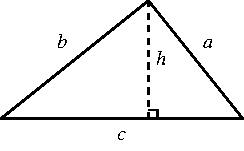
\includegraphics{papers/basel/images/rechtwinklig.pdf}
\caption{Rechtwinkliges Dreieck mit Katheten $a$, $b$, Hypotenuse $c$
und Höhe $h$ auf die Hypotenuse.}
\end{figure}



\subsubsection{Schritt 1: Fläche des Dreiecks}
Das Produkt der Kathetenlängen $ab$ entspricht der Fläche eines Rechtecks,
das genau doppelt so gross ist wie das Dreieck.

%
% rechteck.tex
%
% (c) 2026 Prof Dr Andreas Müller
%
\begin{figure}
\centering

\includegraphics{papers/basel/images/rechteck.pdf}
\caption{Schritt 1: Das Dreieck (grau) hat den halben Flächeninhalt
des Rechtecks mit den Seiten $a$ und $b$.}
\end{figure}


\subsubsection{Schritt 2: Höhe auf die Hypotenuse}
Die Höhe $h$ wird auf die Hypotenuse $c$ gefällt.
Auch dieser Ausdruck verdoppelt die Dreiecksfläche, woraus folgt:
\[
ab = ch.
\]

%
% hoehe.tex
%
% (c) 2026 Prof Dr Andreas Müller
%
\begin{figure}
\centering
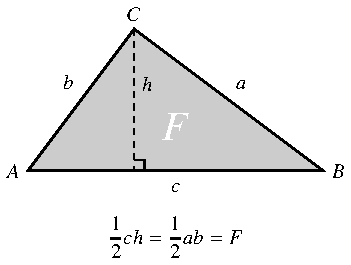
\includegraphics{papers/basel/images/hoehe.pdf}
\caption{Schritt 2: Die Höhe $h$ auf die Hypotenuse $c$ ergibt dieselbe
Dreiecksfläche wie das Produkt der Katheten: $ch = ab$.}
\end{figure}



\subsubsection{Schritt 3: Kehrwerte der Katheten}
Nun wird die Summe der quadratischen Kehrwerte der Katheten berechnet:
\[
\frac{1}{a^2} + \frac{1}{b^2}
=
\frac{a^2 + b^2}{a^2 b^2}
=
\frac{c^2}{c^2 h^2}
=
\frac{1}{h^2}.
\]
Die Summe der quadratischen Kehrwerte der Katheten ist also gleich dem
quadratischen Kehrwert der Höhe auf die Hypotenuse \cite{basel:Wikipedia2}.

%
% katheten.tex
%
% (c) 2026 Prof Dr Andreas Müller
%
\begin{figure}
\centering
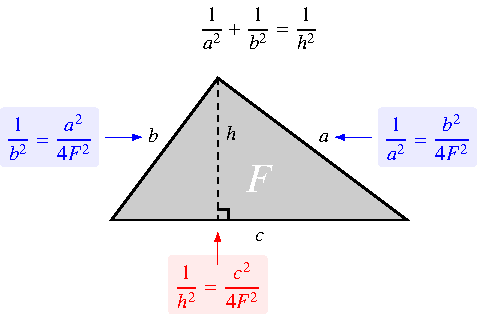
\includegraphics{papers/basel/images/katheten.pdf}
\caption{Schritt 3: Die quadratischen Kehrwerte der Katheten $\frac{1}{a^2}$
und $\frac{1}{b^2}$ (blau) addieren sich zum quadratischen Kehrwert
der Höhe $\frac{1}{h^2}$ (rot).}
\end{figure}


\subsection{Der Konstruktionsprozess}
\label{basel:subsection:konstruktionsprozess}

{\sloppy
Der Beweis benutzt den physikalischen Begriff der \emph{Intensität}:
\index{Intensitat@Intensität}%
Stellt man sich eine Lichtquelle am Punkt $P$ vor, so empfängt
ein Beobachter am Punkt $Z$ eine Helligkeit, die mit dem
Quadrat des Abstands abnimmt:
\[
I(P) \;=\; \frac{1}{|PZ|^2}.
\]
Dies ist das bekannte Abstandsquadratgesetz der Optik.
Die Intensität ist also der quadratische Kehrwert des Abstands von $P$ zu $Z$.
Die zentrale Idee des Beweises ist, dass bei jedem Konstruktionsschritt
jede Lichtquelle durch zwei neue Lichtquellen ersetzt wird, die dieselbe
Eigenintensität (Helligkeit als Quelle) besitzen wie die ursprüngliche.
Da die neuen Quellen weiter von $Z$ entfernt sind, ist die in $Z$
wahrgenommene Intensität jeder einzelnen geringer, aber die in $Z$
wahrgenommene Gesamtintensität bleibt stets erhalten.
Am Ende lässt sich diese erhaltene Gesamtintensität mit der gesuchten Reihe
gleichsetzen \cite{basel:Wikipedia}.
}

\subsubsection{Schritt 1: Ausgangskreis $k_0$}
Man startet mit einem Kreis $k_0$ um den Mittelpunkt $M_0$, der den Umfang~$2$ hat.
Auf dem Kreis liegt unten der Punkt $Z$, genau gegenüber oben der Punkt $M_1$.
Der Durchmesser ergibt sich aus dem Umfang:
\[
U = 2 = \pi d
\quad\Rightarrow\quad
%\implies
d = \frac{2}{\pi} = |M_1 Z|.
\]
Alle folgenden Intensitäten werden bezüglich des Punktes $Z$ berechnet;
$Z$ taucht daher im Index nicht auf.
Die Intensität von $M_1$ beträgt
\[
I(M_1)
=
\frac{1}{|M_1 Z|^2}
=
\frac{1}{d^2}
=
\frac{1}{\biggl(\dfrac{2}{\pi}\biggr)^2}
=
\frac{\pi^2}{4}.
\]

%
% ausgangskreis.tex
%
% (c) 2026 Prof Dr Andreas Müller
%
\begin{figure}
\centering
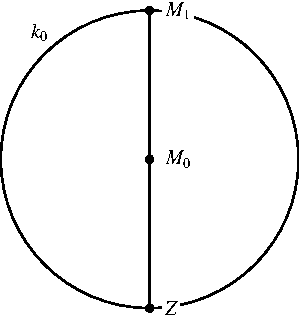
\includegraphics{papers/basel/images/ausgangskreis.pdf}
\caption{Ausgangskreis $k_0$ mit Umfang 2, Mittelpunkt $M_0$,
oberem Punkt $M_1$ und unterem Punkt $Z$.}
\end{figure}


\subsubsection{Schritt 2: Erster Konstruktionskreis $k_1$}
Es wird ein weiterer Kreis $k_1$ um $M_1$ mit Radius $|M_1 Z|$ gezeichnet.
Durch $M_1$ legt man eine Senkrechte zu $\overline{ZM_1}$, wodurch die
Punkte $P_{1,1}$ und $P_{1,2}$ entstehen.

%
% k1.tex
%
% (c) 2026 Prof Dr Andreas Müller
%
\begin{figure}
\centering
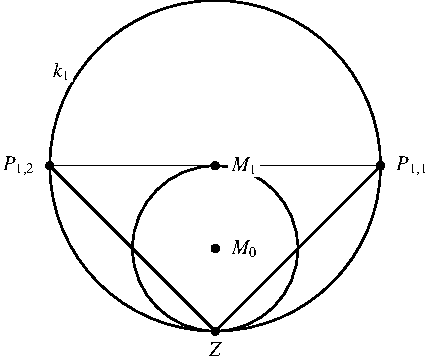
\includegraphics{papers/basel/images/k1.pdf}
\caption{Erster Konstruktionsschritt: Kreis $k_1$ um $M_1$ mit den Punkten
$P_{1,1}$ und $P_{1,2}$. Bogenlängen: $P_{1,1}P_{1,2} = 2$, $P_{1,2}Z = 1$,
$ZP_{1,1} = 1$.}
\end{figure}


\subsubsection{Schritt 3: Intensitäten auf $k_1$}
Aus $P_{1,1}$, $P_{1,2}$ und $Z$ entsteht nach dem Satz des Thales ein
rechtwinkliges Dreieck mit rechtem Winkel bei $Z$.
$M_1$ ist der Höhenfusspunkt in diesem Dreieck.
Die einzelne Lichtquelle bei $M_1$ wird nun durch zwei Lichtquellen
bei $P_{1,1}$ und $P_{1,2}$ ersetzt, die jeweils dieselbe Eigenintensität
(d.\,h. dieselbe Helligkeit als Lichtquelle) besitzen wie die ursprüngliche
Quelle bei $M_1$.
Da $P_{1,1}$ und $P_{1,2}$ weiter von $Z$ entfernt sind als $M_1$, empfängt $Z$
von jeder dieser Quellen weniger Licht. Die in $Z$ wahrgenommene Gesamtintensität
bleibt jedoch nach dem inversen Satz des Pythagoras erhalten:
\[
I(M_1) = \frac{\pi^2}{4} = I(P_{1,1}) + I(P_{1,2}).
\]

\subsubsection{Schritt 4: Zweiter Konstruktionskreis $k_2$}
Um $M_2$ wird ein Kreis $k_2$ mit Radius $|M_2 Z|$ gezeichnet.
Die Gerade durch $M_2$ und $P_{1,1}$ schneidet $k_2$ in den Punkten
$P_{2,1}$ und $P_{2,3}$; die Gerade durch $M_2$ und $P_{1,2}$ liefert
entsprechend $P_{2,2}$ und $P_{2,4}$.

\subsubsection{Schritt 5: Intensitäten auf $k_2$}
Das Dreieck $P_{2,1}P_{2,3}Z$ ist nach dem Satz des Thales rechtwinklig
bei $Z$, und $P_{1,1}$ ist der Höhenfusspunkt.
Die Lichtquelle bei $P_{1,1}$ wird durch zwei Lichtquellen bei $P_{2,1}$
und $P_{2,3}$ ersetzt, die dieselbe Eigenintensität besitzen wie die
ursprüngliche Quelle bei $P_{1,1}$.
Da $P_{2,1}$ und $P_{2,3}$ weiter von $Z$ entfernt sind als $P_{1,1}$,
ist die in $Z$ wahrgenommene Intensität jeder einzelnen neuen Quelle geringer.
Die in $Z$ wahrgenommene Gesamtintensität bleibt jedoch erhalten:
\[
I(P_{1,1}) = I(P_{2,1}) + I(P_{2,3}).
\]
Analog wird die Lichtquelle bei $P_{1,2}$ durch zwei Lichtquellen
bei $P_{2,2}$ und $P_{2,4}$ ersetzt, die dieselbe Eigenintensität besitzen
wie die ursprüngliche Quelle bei $P_{1,2}$, wobei $P_{1,2}$ der Höhenfusspunkt im
Dreieck $P_{2,2}P_{2,4}Z$ ist:
$I(P_{1,2}) = I(P_{2,2}) + I(P_{2,4})$.
Insgesamt bleibt die Gesamtintensität erhalten:
\[
I(P_{1,1}) + I(P_{1,2})
=
I(P_{2,1}) + I(P_{2,2}) + I(P_{2,3}) + I(P_{2,4})
=
\frac{\pi^2}{4}.
\]
Da $k_2$ doppelt so gross ist wie $k_1$ (Umfang~$8$), liegen die Punkte
äquidistant. Die Bogenlängen betragen:
\[
\widehat{ZP_{2,1}} = 1,\quad
\widehat{P_{2,1}P_{2,2}} = 2,\quad
\widehat{P_{2,2}P_{2,3}} = 2,\quad
\widehat{P_{2,3}P_{2,4}} = 2,\quad
\widehat{P_{2,4}Z} = 1.
\]

% 
%
%
% k2.tex
%
% (c) 2026 Prof Dr Andreas Müller
%
\begin{figure}
\centering
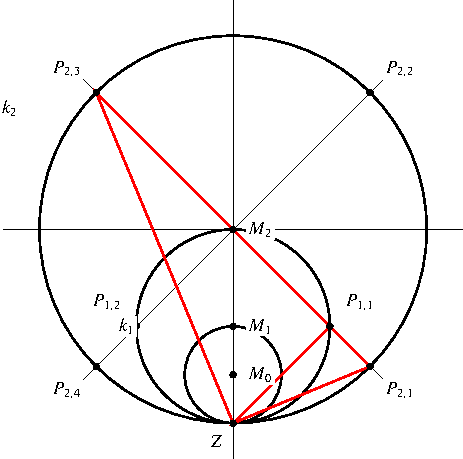
\includegraphics{papers/basel/images/k2.pdf}
\caption{Zweiter Konstruktionsschritt: Kreis $k_2$ mit den Punkten
$P_{2,1}$, $P_{2,2}$, $P_{2,3}$, $P_{2,4}$.}
\end{figure}


\subsubsection{Schritt 6: Dritter Konstruktionskreis $k_3$ und Invarianten}
Um $M_3$ wird ein Kreis $k_3$ mit Radius $|M_3 Z|$ gezeichnet.
Als Beispiel: das Dreieck $P_{3,2}P_{3,6}Z$ ist nach dem Satz des Thales
rechtwinklig bei $Z$, und $P_{2,2}$ ist der zugehörige Höhenfusspunkt.
Die Lichtquelle bei $P_{2,2}$ wird durch zwei Lichtquellen bei $P_{3,2}$
und $P_{3,6}$ ersetzt, die dieselbe Eigenintensität besitzen wie die
ursprüngliche Quelle bei $P_{2,2}$. Da diese weiter von $Z$ entfernt sind,
ist die in $Z$ wahrgenommene Intensität jeder einzelnen neuen Quelle geringer.
Die in $Z$ wahrgenommene Gesamtintensität bleibt jedoch erhalten.
Dasselbe gilt für jeden Punkt auf $k_2$, sodass alle Lichtquellen durch
Lichtquellen gleicher Eigenintensität auf $k_3$ ersetzt werden.
Dabei bleiben bei jedem Schritt zwei Grössen konstant:
\begin{itemize}
  \item Die Summe aller Intensitäten auf dem jeweiligen Kreis beträgt stets
        $\dfrac{\pi^2}{4}$.
  \item Die Punkte liegen äquidistant mit konstanter Bogenlänge~$2$.
\end{itemize}

% 
%
%
% k3.tex
%
% (c) 2026 Prof Dr Andreas Müller
%
\begin{figure}
\centering
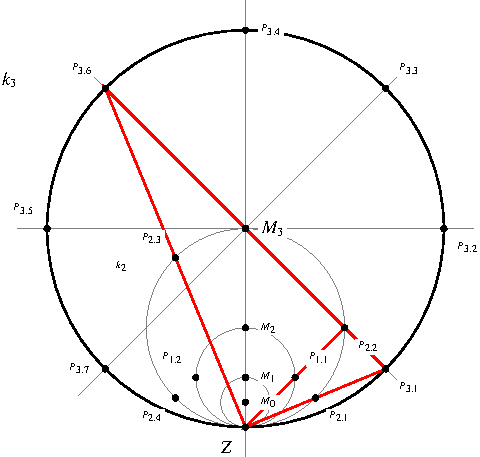
\includegraphics{papers/basel/images/k3.pdf}
\caption{Dritter Konstruktionsschritt: Kreis $k_3$ mit acht
äquidistanten Punkten.}
\end{figure}


\subsection{Der Grenzübergang}
\label{basel:subsection:grenzuebergang}

%
% zahlengerade.tex
%
% (c) 2026 Prof Dr Andreas Müller
%
\begin{figure}
\centering
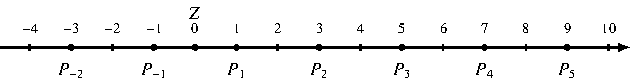
\includegraphics{papers/basel/images/zahlengerade.pdf}
\caption{Grenzübergang: Der Kreis $k_n$ wird zur Zahlengeraden durch $Z = 0$.
Die Punkte $P_k$ liegen bei den ungeraden Zahlen
$\ldots, -3, -1, 1, 3, 5, \ldots$
im Abstand $1, 3, 5, 7, \ldots$ von $Z$.
\label{basel:figure:gerade}}
\end{figure}

 
\subsubsection{Schritt 7: Übergang zur Geraden}
Im Grenzübergang $n \to \infty$ wächst der Kreis $k_n$ ins Unendliche und
wird zu einer Geraden durch $Z$ (Abbildung~\ref{basel:figure:gerade}).
Da die Bogenlängen konstant $1, 2, 2, \ldots$ betragen, liegen die Punkte
auf dieser Geraden im Abstand $1, 3, 5, 7, \ldots$ zu beiden Seiten von $Z$.

\subsubsection{Schritt 8: Gesamtintensität und Symmetrie}
Die Summe aller Intensitäten bleibt auch im Grenzwert erhalten:
\[
    \bigl( I(P_1) + I(P_2) + I(P_3) + \cdots \bigr)
    +
    \bigl( I(P_{-1}) + I(P_{-2}) + I(P_{-3}) + \cdots \bigr)
    =
    \frac{\pi^2}{4}.
\]
Wegen der Symmetrie der Konstruktion gilt für jede Seite:
\[
    I(P_1) + I(P_2) + I(P_3) + \cdots = \frac{\pi^2}{8}.
\]

\subsubsection{Schritt 9: Explizite Reihe für ungerade Zahlen}
Da die Punkte im Abstand $1, 3, 5, 7, \ldots$ von $Z$ liegen und die
Intensität mit dem Quadrat des Abstands abnimmt, ergibt sich:
\[
S_u
=
\frac{1}{1^2} + \frac{1}{3^2} + \frac{1}{5^2} + \frac{1}{7^2} + \cdots
=
\frac{\pi^2}{8}.
\]

\subsubsection{Schritt 10: Vollständige Reihe und Ergebnis}
Die vollständige Reihe $S$ setzt sich aus dem Anteil der ungeraden Zahlen
$S_u$ und dem Anteil der geraden Zahlen $S_g$ zusammen:
\[
S
=
\frac{1}{1^2} + \frac{1}{2^2} + \frac{1}{3^2} + \frac{1}{4^2} + \cdots
=
S_u + S_g.
\]
Der gerade Anteil lässt sich auf $S$ zurückführen:
\[
S_g
=
\frac{1}{2^2} + \frac{1}{4^2} + \frac{1}{6^2} + \cdots
=
\frac{1}{4}
\biggl(
\frac{1}{1^2} + \frac{1}{2^2} + \frac{1}{3^2} + \cdots
\biggr)
=
\frac{1}{4} S.
\]
Einsetzen liefert
\[
S
=
\frac{\pi^2}{8} + \frac{1}{4} S
\quad\Rightarrow\quad
%\implies
\frac{3}{4} S = \frac{\pi^2}{8}
\quad\Rightarrow\quad
%\implies
S = \frac{\pi^2}{8} \cdot \frac{4}{3}
\]
und damit das gesuchte Ergebnis:
\begin{equation*}
S = \frac{\pi^2}{6}.
%\label{basel:equation:geometrie-ergebnis}
\end{equation*}

In dem YouTube-Video \textit{Why is pi here? And why is it squared? A geometric answer 
to the Basel problem} von 3Blue1Brown \cite{Basel:YouTube2} wird dieser Beweis ebenfalls 
sehr gut und anschaulich erklärt.
